Se analizarán los resultados obtenidos con respecto al tiempo de ejecución y memoria utilizada al realizar de manera práctica cada algoritmo. Los valores de la memoria usada representan el peak de memoria adicional observado durante la ejecución de cada algoritmo, tomando muestras cada $0,1$ ms, por lo que un valor de $0$ KB no significa que el algoritmo no utilice memoria auxiliar, sino que no se detectó un aumento adicional durante cada muestra tomada.

\subsection{Algoritmos de ordenamiento}

Mencionar que para el algoritmo de Quick Sort, fue tomado como pivote la mitad del arreglo que se este analizando, esto ya que en el código de la fuente en la cual se extrajo el algoritmo, se usaba el pivote en uno de los peores casos y es muy ineficiente (pivote al inicio o final en arreglos de orden ascendente o descendente).

Al ejecutar los algoritmos de ordenamiento con un dominio D7 y ordenado de forma aleatoria, se obtienen los siguientes gráficos:

\begin{figure}[H]
    \centering

    \begin{minipage}{0.48\textwidth}
        \centering
        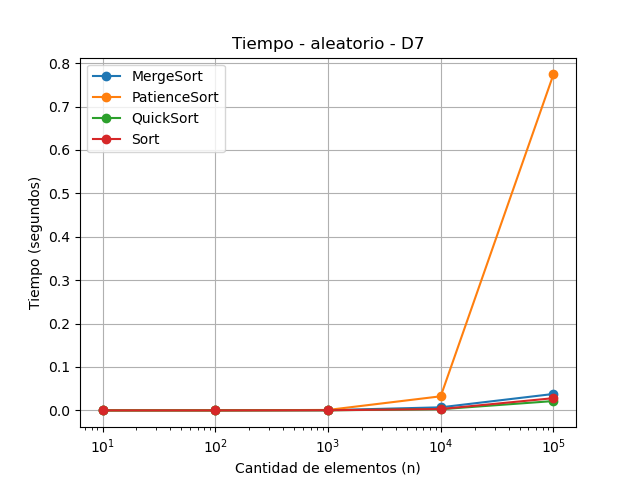
\includegraphics[width=0.85\textwidth]{figures/tiempo_aleatorio_D7.png}
        \caption*{Tiempo de ejecución}
    \end{minipage}
    \hfill
    \begin{minipage}{0.48\textwidth}
        \centering
        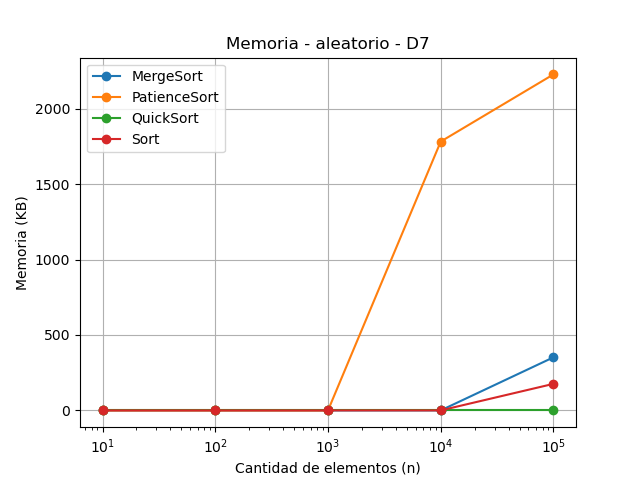
\includegraphics[width=0.85\textwidth]{figures/memoria_aleatorio_D7.png}
        \caption*{Memoria utilizada}
    \end{minipage}

    \caption{Tiempo y memoria utilizada en sorting con dominio D7 y orden aleatorio.}
    \label{fig:comparacion_sorting}
\end{figure}

En la Figura 1 se observa que Patience Sort presenta el mayor crecimiento temporal, alcanzando aproximadamente $0,78$ s para $n=10^5$, esto se debe a que su implementación puede aproximarse a $O(n^2)$, ya que para decidir en qué pila insertar cada elemento, se recorren linealmente las pilas existentes y luego, durante el proceso de reconstrucción del arreglo ordenado a partir de las pilas, se vuelve a buscar repetidamente el menor elemento entre los topes de las pilas. En cambio, Merge Sort, Quick Sort y Sort mantienen tiempos considerablemente menores: Merge Sort divide siempre el arreglo en mitades, Quick Sort obtiene particiones relativamente balanceadas en este caso por como se colocó el pivote, y Sort utiliza una implementación optimizada, por lo que los tiempos promedios de estos 3 algoritmos se mantienen cercanos a un comportamiento de $O(n\log n)$.

Con respecto a la memoria, Patience Sort también presenta el mayor consumo debido a la utilización de múltiples pilas, ya que debe mantener guardados los elementos distribuidos usando una estructura de tipo \verb|vector<vector<int>>|, teniendo una complejidad espacial $O(n)$. Merge Sort también utiliza $O(n)$ debido a los arreglos auxiliares que crea para almacenar de forma temporal las mitades durante el proceso de mezcla. En el caso de Quick Sort, este trabaja principalmente sobre el mismo arreglo, pero a pesar de esto no es estrictamente in-place, debido a la memoria adicional proveniente en mayor parte de las llamadas recursivas (almacenando cosas como parámetros, la variable pivote, entre otros elementos), siendo aproximadamente $O(\log n)$ cuando las particiones se mantienen balanceadas. Finalmente, Sort también trabaja principalmente sobre el mismo arreglo y utiliza una cantidad escasa de memoria auxiliar, por lo que el consumo observado en estos 2 ultimos algortimos es menor en comparación con Patience Sort y Merge Sort.

Ahora, si vemos los gráficos de memoria vs n y tiempo vs n con arreglo aleatorio pero con dominio D1, se puede observar lo siguiente:

\begin{figure}[H]
    \centering

    \begin{minipage}{0.48\textwidth}
        \centering
        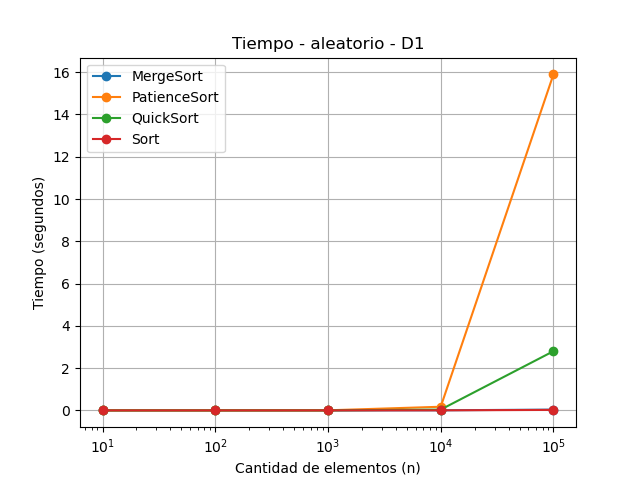
\includegraphics[width=0.85\textwidth]{figures/tiempo_aleatorio_D1.png}
        \caption*{Tiempo de ejecución}
    \end{minipage}
    \hfill
    \begin{minipage}{0.48\textwidth}
        \centering
        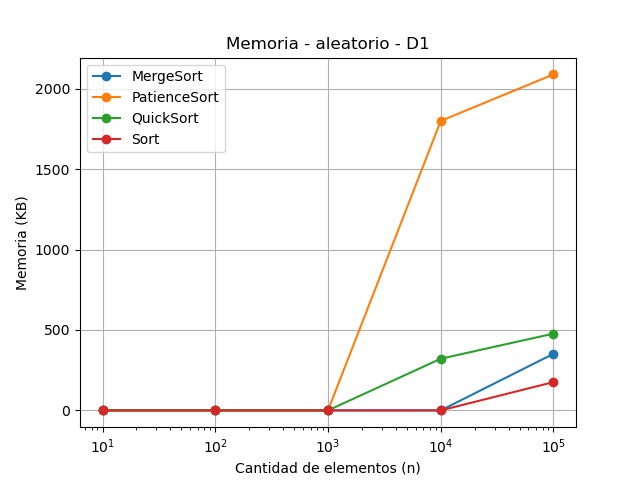
\includegraphics[width=0.85\textwidth]{figures/memoria_aleatorio_D1.png}
        \caption*{Memoria utilizada}
    \end{minipage}

    \caption{Tiempo y memoria utilizada en sorting con dominio D1 y orden aleatorio.}
    \label{fig:comparacion_sorting}
\end{figure}

Al comparar los resultados de D1 y D7 para arreglos aleatorios mostrados en la figura 1 y 2, se observa que el dominio afecta principalmente a Patience Sort y Quick Sort. Para $n=10^5$, ya que Patience Sort aumenta desde aproximadamente $0.78$ segundos en D7 hasta cerca de $16$ segundos en D1. Esto debido a que D1 genera una mayor cantidad de valores repetidos, lo que conlleva la creación de más pilas en Patience Sort y aumenta el costo de reconstrucción del arreglo ordenado.

Quick Sort también empeora en D1, ya que los valores repetidos pueden producir particiones menos balanceadas y por ende, una mayor cantidad de llamadas recursivas. En cambio, Merge Sort y Sort presentan un comportamiento más estable entre ambos dominios.

Respecto a la memoria, Patience Sort mantiene el mayor consumo debido al uso de múltiples pilas. Quick Sort es el que mayormente cambia en comparación a D7, ya que presenta un mayor uso de memoria en D1, esto se asocia a una mayor profundidad de recursión, mientras que Merge Sort y Sort muestran variaciones menores.

Al comparar los arreglos ascendentes y descendentes, se obtuvieron los siguientes gráficos con dominio D7:

\begin{figure}[H]
    \centering

    \begin{minipage}{0.48\textwidth}
        \centering
        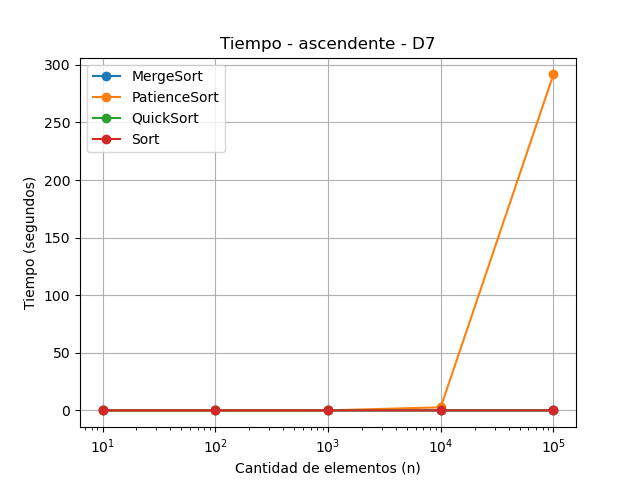
\includegraphics[width=0.85\textwidth]{figures/tiempo_ascendente_D7.png}
        \caption*{Tiempo de ejecución}
    \end{minipage}
    \hfill
    \begin{minipage}{0.48\textwidth}
        \centering
        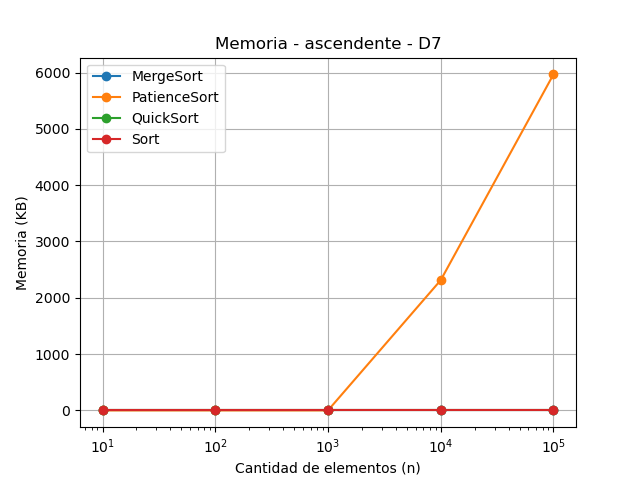
\includegraphics[width=0.85\textwidth]{figures/memoria_ascendente_D7.png}
        \caption*{Memoria utilizada}
    \end{minipage}

    \caption{Tiempo y memoria utilizada en sorting con dominio D7 y orden ascendente.}
    \label{fig:comparacion_sorting}
\end{figure}

\begin{figure}[H]
    \centering

    \begin{minipage}{0.48\textwidth}
        \centering
        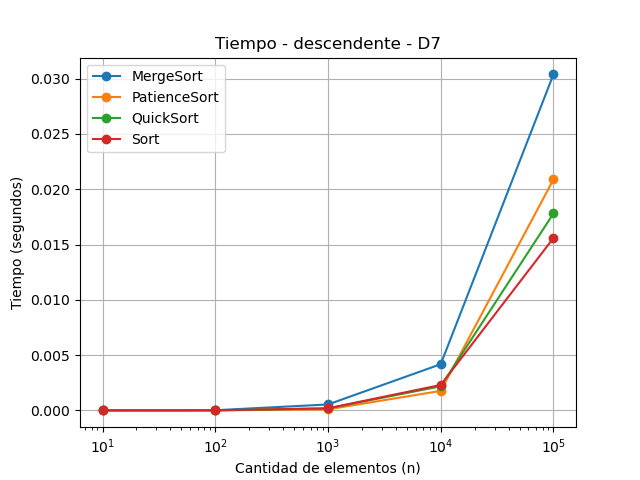
\includegraphics[width=0.85\textwidth]{figures/tiempo_descendente_D7.png}
        \caption*{Tiempo de ejecución}
    \end{minipage}
    \hfill
    \begin{minipage}{0.48\textwidth}
        \centering
        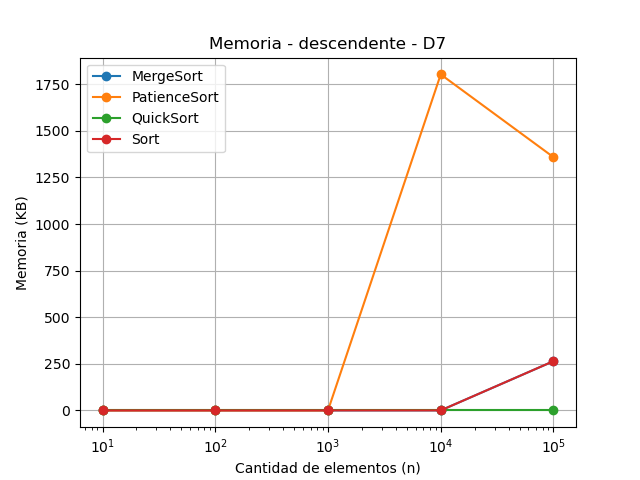
\includegraphics[width=0.85\textwidth]{figures/memoria_descendente_D7.png}
        \caption*{Memoria utilizada}
    \end{minipage}

    \caption{Tiempo y memoria utilizada en sorting con dominio D7 y orden descendente.}
    \label{fig:comparacion_sorting}
\end{figure}

En la figura 4, la principal diferencia se puede ver en Patience Sort, ya que en los arreglos ascendentes, su implementación puede acercarse a un comportamiento de $O(n^2)$, debido a la creación muchas pilas que luego deben recorrerse repetidamente. En cambio, en los arreglos descendentes todos los valores se van guardando casi en la misma pila por lo que el tiempo disminuye considerablemente.

Quick Sort presenta un comportamiento cercano a $O(n \log n)$ cuando las particiones son balanceadas, mientras que Merge Sort mantiene $O(n \log n)$ independientemente del orden inicial. Sort también tiene un comportamiento cercano a $O(n \log n)$ debido a que este algoritmo en las librerías de c++, está optimizado.

Respecto a la memoria, Patience Sort presenta el mayor consumo (al crear tantas pilas), con complejidad espacial $O(n)$. Merge Sort también utiliza $O(n)$ por sus arreglos auxiliares, mientras que Quick Sort utiliza principalmente memoria asociada a la recursión, aproximadamente $O(\log n)$ en un caso balanceado. Finalmente, Sort también trabaja principalmente sobre el mismo arreglo y utiliza poca memoria auxiliar, por lo que su consumo adicional se mantiene bajo.

Un caso especial se observa en el gráfico descendente D7, donde Patience Sort presenta un menor tiempo de ejecución que Merge Sort, ya que esta distribución ayuda a la formación de pocas pilas.

\subsection{Multiplicación de Matrices}

Se realizará un análisis unicamente de matrices densas con dominio D10, esto ya que los resultados obtenidos en matrices diagonales y dispersas son muy parecidos, además de que las matrices densas son el caso más general para representar la multiplicación de matrices, debido a que la mayoría de las posiciones tienen valores distintos de cero en la práctica.

\begin{figure}[H]
    \centering

    \begin{minipage}{0.48\textwidth}
        \centering
        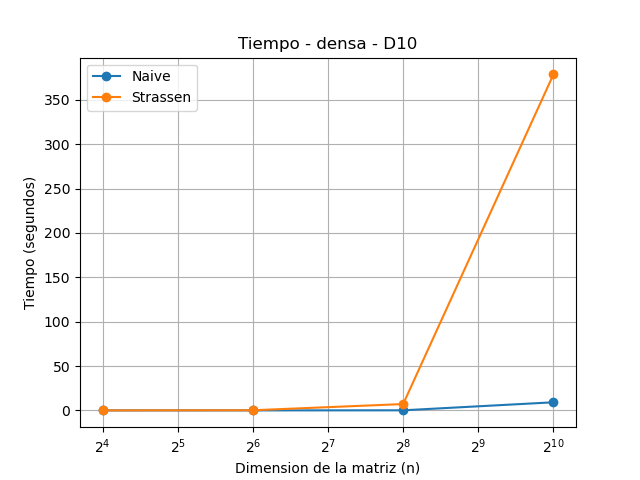
\includegraphics[width=0.85\textwidth]{figures/tiempo_densa_D10.png}
        \caption*{Tiempo de ejecución}
    \end{minipage}
    \hfill
    \begin{minipage}{0.48\textwidth}
        \centering
        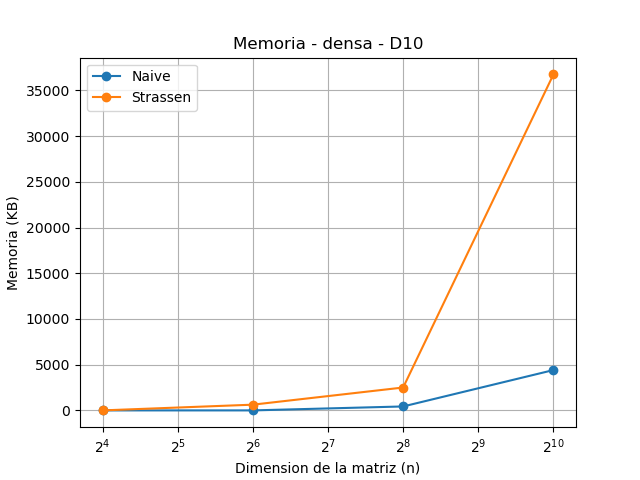
\includegraphics[width=0.85\textwidth]{figures/memoria_densa_D10.png}
        \caption*{Memoria utilizada}
    \end{minipage}

    \caption{Tiempo y memoria utilizada en matrix\_multiplication con dominio D10 y tipo de matriz densa.}
    \label{fig:comparacion_sorting}
\end{figure}

En la figura 5 se ve que aunque Strassen posee una complejidad temporal teórica de $O(n^{2.807})$, menor que el $O(n^3)$ del método Naive, esta disminición se debe a que en la ecuación de recurrencia del método Strassen, se logra reducir de 8 a 7 subproblemas de multiplicación de matrices. A pesar de esto, en los tamaños evaluados Strassen presenta tiempos bastante mayores. Esto se debe al costo práctico de las llamadas recursivas y de la creación de numerosas matrices auxiliares. Por lo que, para estos tamaños, la ventaja asintótica de Strassen todavía no compensa ese costo adicional.

Con respecto a la memoria, ambos algoritmos presentan un crecimiento de orden $O(n^2)$, pero Strassen utiliza más memoria debido a las submatrices y estructuras auxiliares creadas durante la recursión.

Además, a medida que aumentan la dimensiones de las matrices, la diferencia entre ambos algoritmos se vuelve más evidente. Para $n=2^{10}$, Strassen alcanza aproximadamente $370$ segundos, mientras que Naive se mantiene cerca de los $8$ segundos. Esto muestra que, aunque Strassen tenga una mejor complejidad asintótica, para los tamaños analizados el costo de dividir las matrices, realizar las llamadas recursivas y crear estructuras auxiliares es demasiado alto como para superar al método Naive. Es decir, una mejor complejidad asintótica no conlleva necesariamente un menor tiempo de ejecución para todos los casos.

Esta diferencia entre ambos algoritmos, también se observa en memoria, para $n=2^{10}$, Strassen alcanza un peak cercano a $37000$ KB, mientras que Naive utiliza alrededor de $4000$ KB adicionales. Esto se debe a que Naive trabaja principalmente con las matrices originales y la matriz resultado, mientras que Strassen genera múltiples submatrices y matrices auxiliares durante cada nivel de recursión.
